\newpage
\subsection{Drehstromtrafo}
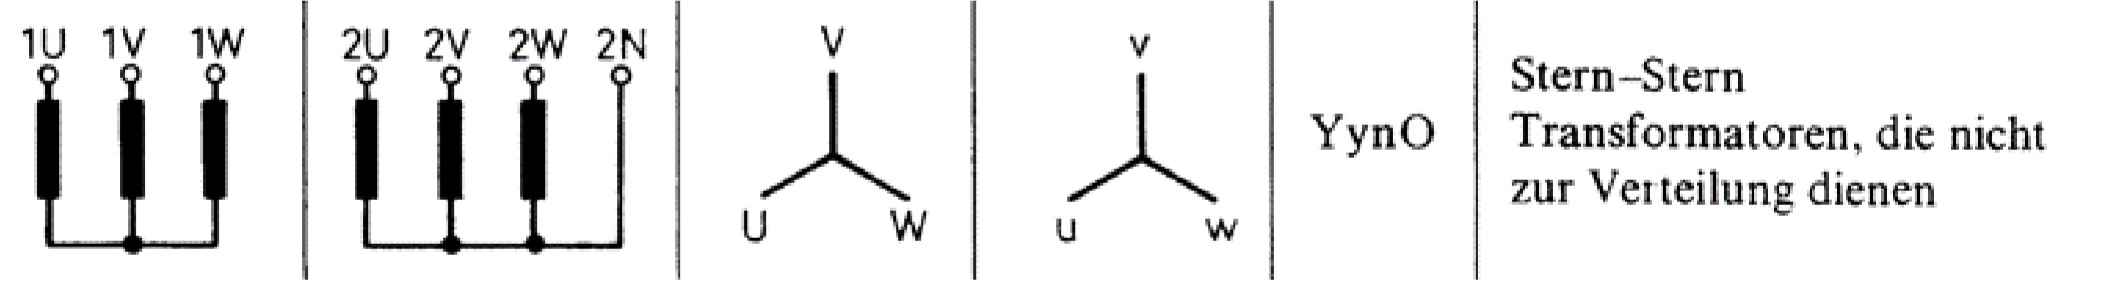
\includegraphics[width=0.99\textwidth]{bilder/a71.png}

\begin{minipage}{0.49\textwidth}
Von dem Trafo sind folgende Daten bekannt:
\begin{itemize}
\itemsep0em
\item Nennleistung $S_{1N} = 30MVA$
\item Primärnennspannung $ U_{1N} = 30kV / 50Hz$
\item Sekundärnennspannung $ U_{2N} = 10kV / 50Hz$ 
\item Windungszahlen je Strang $N_1 = 288$, $N_2 = 96$
\item Leerlaufstrom $I_{10} = 3.5A$
\item Leerlaufwirkleistung $P_{10} = 50.6kW$
\item Kurzschlussspannung $U_{1K} = 2700V$
\item Kurzschlusswirkleistung $P_{1K} = 152kW$
\end{itemize}
\end{minipage}
\begin{minipage}{0.49\textwidth}
\textbf{Einphasiges Ersatzschaltbild}

\adjustbox{width=0.8\textwidth}{\begin{circuitikz}[european]
	\draw (0,0) coordinate (In1) {} 
		to[short, *-, i=$\underline{I_1}$] ++(1,0)
		to[R, l=$R_1$] ++(2,0)
		to[L, l=$jX_{\sigma 1}$] ++(2,0)
		to[short, -*] ++(1,0) coordinate (middle1) {}
		to[short] ++(1,0)
		to[L, l=$jX'_{\sigma 2}$] ++(2,0)
		to[R, l=$R'_2$] ++(2,0)
		to[short, -* ,i<=$\underline{I_2}$] ++(1,0) coordinate(Out1);
	\draw (middle1) to[short, -*] ++(0,-1) coordinate (middle2) {};
	\draw (middle2) -- ++(-1,0) 
		to[R, l=$R_{Fe}$] ++(0,-2)
		to[short, -*] ++(1,0) coordinate(middle3)
		to[short, -*] ++(0,-1) coordinate(middle4);
	\draw (middle2) -- ++(1,0)
		to[L, l=$jX_h$] ++(0,-2)
		to[short] (middle3);
	\draw (middle4) to[short, -*] ++(-6,0) coordinate(In2);
	\draw (middle4) to[short, -*] ++(6,0) coordinate(Out2);
	\begin{scope}[
		shorten <=10pt,
		shorten >= 10pt,
		->
	]
		\draw (In1) -- (In2) node[midway, right] {$\underline{U_1}$};
		\draw (Out1) -- (Out2) node[midway, left] {$\underline{U'_2}$};
	\end{scope}
\end{circuitikz}}

\textbf{Einphasiges Ersatzschaltbild Leerlauf}

\adjustbox{width=0.6\textwidth}{\begin{circuitikz}[european]
	\draw (0,0) coordinate (In1) {} 
		to[short, *-, i=$\underline{I}_{10}$] ++(1,0)
		to[R, l=$R_1$] ++(2,0)
		to[L, l=$jX_{\sigma 1}$] ++(2,0)
		to[short, -*] ++(1,0) coordinate (middle1) {}
		to[short, -* ,i<=\mbox{$\underline{I}_2 = 0$}] ++(3,0) coordinate(Out1);
	\draw (middle1) to[short, -*] ++(0,-1) coordinate (middle2) {};
	\draw (middle2) 
		to[short, i_=$\underline{I}_{1Fe}$] ++(-1,0) 
		to[R, l=$R_{Fe}$] ++(0,-2)
		to[short, -*] ++(1,0) coordinate(middle3)
		to[short, -*] ++(0,-1) coordinate(middle4);
	\draw (middle2) 
		to[short, i=$\underline{I}_{1\mu}$] ++(1,0)
		to[L, l=$jX_h$] ++(0,-2)
		to[short] (middle3);
	\draw (middle4) to[short, -*] ++(-6,0) coordinate(In2);
	\draw (middle4) to[short, -*] ++(3,0) coordinate(Out2);
	\begin{scope}[
		shorten <=10pt,
		shorten >= 10pt,
		->
	]
		\draw (In1) -- (In2) node[midway, right] {$\underline{U}_{10}$};
		\draw (Out1) -- (Out2) node[midway, right] {$\underline{U}'_{20}$};
	\end{scope}
\end{circuitikz}}
\end{minipage}


\begin{enumerate}
\item Leerlaufberechnungen
\begin{align*}
	S_l &= \sqrt{3} \cdot U\cdot I = \sqrt{3} \cdot 30'000V\cdot 3.5A = 181.865kVA\\
	Q_L&= \sqrt{S_L^2-P_L^2} = \sqrt{(181.865kVA)^2-(50.6kW)^2} = 174.684kVAr\\
	&\textrm{Vernachlässigen von }R_1 \textrm{ und } X_{\sigma1}\\
	R_{FE}&=\frac{U_{10}^2}{P_{10}} = \frac{(30kV)^2}{50.6kW} = 17'786.8\Omega\\
	X_H &= \frac{U_{10}^2}{Q_L} = \frac{(30kV)^2}{174.684kVAr} = 5152.14\Omega\\
	L_H &= \frac{X_H}{\omega} = \frac{17.787k\Omega}{100\pi} = 16.399H
\end{align*}
\item Kurzschlussberechnungen
\begin{align*}
	I_{1N - 1\textrm{Phase}} &= \frac{30MVA}{3}\cdot \frac{\sqrt{3}}{30kVA} = 577.35A\\
	Z_K &= \frac{U_K}{\sqrt{3}}\cdot \frac{1}{I_{1N}} = \frac{2700}{\sqrt{3}\cdot 577.35A} = 2.7\Omega	\\
	P_K &= \sqrt{3}\cdot I_k^2\cdot R \Rightarrow R =\frac{P_k}{\sqrt{3}\cdot I_k^2} = \frac{152kW}{\sqrt{3}\cdot (577.35A)^2} = 0.152\Omega\\
	X_K &= \sqrt{Z^2 - R^2} = 2.6957\Omega\\
	Z &= (0.152+j\cdot 2.6957)\Omega
\end{align*}
\item Belastungsberechnungen
\begin{align*}
R_{2N}&= \frac{U^2_{2N}}{S_{2N}} = \frac{(10kV)^2}{30MVA} = 3.333\Omega \Rightarrow R'_2 = R_2\cdot  \left(\frac{288}{96}\right)^2 = 30\Omega\\ 
\underline{U'_2} &= \underline{U_1} - \underline{Z_K} \cdot \frac{\underline{U'_2}}{R'_2} = \frac{\underline{U_1}}{1+\frac{\underline{Z_K}}{R'_{2N}}} = \frac{30kV}{1+\frac{(0.152+j\cdot 2.6957)\Omega}{30\Omega}} = 29730.2V\angle -5.11^\circ\\
U_2 &= U'_2\cdot \frac{N_2}{N_1} = 29730.2V\angle -5.11^\circ \cdot \frac{96}{288} = 9910V\angle -5.11^\circ\\
P_{2N} &= \frac{U_2^2}{R_2} =\frac{(9910.06V)^2}{3.33333\Omega} = 29.462MVA\\
\eta &= \frac{P_2}{P_2+P_{10}+P_K} = \frac{29.462MVA}{29.462MVA+50.6KW+152kW} = 99.3\%
\end{align*}
\end{enumerate}





